\begin{savequote}[75mm]

\end{savequote}

\chapter{Model and Simulation}
{\lettrine[lines=3,slope=1pt,nindent=1pt,]{\textcolor{SchoolColor}{C}}{onsider a $Y \times X$\ \ bounded lattice graph} where $X,Y\in\N$. For simplicity, let $Z = YX$. In each vertex, there is a single residence for a single agent. We allow for vacant houses, hence, there are $Z$ houses and $N$ agents where $N \leq Z$. Agents are defined by a their race, $r\in\{$White, Black, Hispanic$\}$ and income $w$. This paper simplifies the wealth distribution with the function $w(x)\in[1,3]$ where:  
\begin{equation}
\label{eq:w}
    w(x) = \left\{\begin{array}{lr}
        1 & $x$<\$35k\\
        2 & \$35k \leq $x$ \leq \$100k\\
        3 & $x$ >\$100k
        \end{array}\right\}.
\end{equation}
The framework in this model allows for any discrete measure of wealth and race. The wealth levels are smoothed to three levels to simplify to low, medium, and high wealth. Since the model is tailored to Chicago, we exclude Asians, Native Americans, and mixed races, as they represent less than 6\% of the population in Chicago. The Schelling model has difficulty incorporating small minorities in the model. Given that this paper is simulating an aggregate of agents, the Schelling model will not be able to interact the small minority residents in a meaningful manner.

\section{Schelling Segregation}
In the 1971 Schelling model, agents were defined as either an `X' or `O' to indicate their race and are placed onto the board in some random or non-random order. This paper has three distinct races. We define a tolerance level $\tau\in[0,1]$ which is the minimum level that each agent will accept being a minority in their neighborhood. If $\tau = 0.4$, then each agent $i$ of race $r$ will be dissatisfied unless at least 40\% of its neighbors are also of race $r$. Tolerance levels are common across all agents regardless of race. Neighborhoods are Morse Neighborhoods, which are defined by the 8 closest points to the agent on a grid. This is shown in Figure \ref{fig:morse} below. Other Schelling models use Manhattan distance, usually with $d=1$ or $d=2$, as in Figure \ref{fig:MD}. However, Zhang 2011 simulates that changing the neighborhood does not significantly alter the underlying segregation, just the speed of convergence\cite{zhang11}. 

\begin{figure}[h!]
\centering
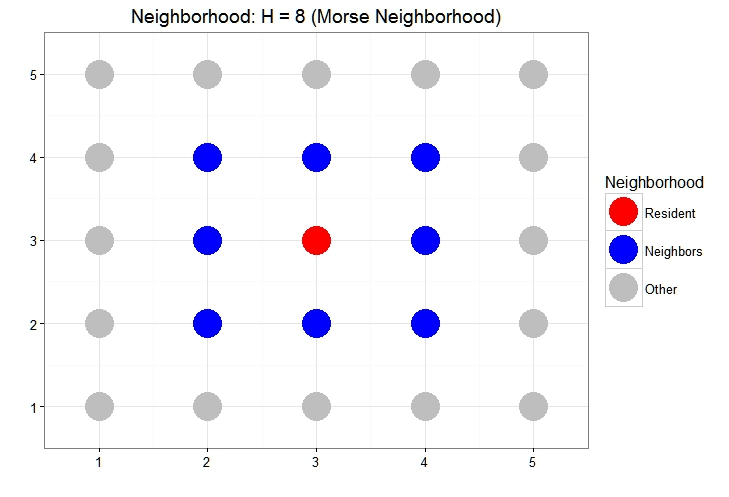
\includegraphics[scale=.33]{figures/H8.jpeg}
\caption{Diagram of Morse Neighborhood}
\label{fig:morse}
\end{figure}

At each step, all the agents simultaneously look at their neighborhood to calculate their ratio of matching race. If that ratio is smaller than the minimum tolerance level, then the agent is \textit{unsatisfied}. All \textit{unsatisfied} agents are simultaneously removed from the board. In Schelling, the agents are placed back into the board randomly, as in Algorithm \ref{alg:euclid}. Luckily, the complexity of the algorithm is $O(n^2)$ at each step. However, at high tolerance levels, the number of steps the algorithm takes grows quickly. For this reason, we run the algorithm until there is at most 10\% \textit{unsatisfied} agents.

 \begin{algorithm}[h!]
  \caption{Schelling Process}\label{alg:euclid}
  \begin{algorithmic}[1]
  	\Function{Schelling}{$agents, grid, tolerance$}\Comment{Agents are defined by their race}
   		\Procedure{Satisfaction}{$agent_i, subgrid, tolerance$}\Comment{The $subgrid$ is a Morse neighborhood of $agent_i$}
        	\State Let $sat = \frac{\text{matching agents in $subgrid$ to $agent_i$}}{\text{size of subgrid}}$
       		\If {$tolerance < sat $}
       			\State return $TRUE$. \Comment{The agent is $satisfied$.}
                \Else \ return $FALSE$. \Comment{The agent is $unsatisfied$.}
    		\EndIf
        \EndProcedure
    	\While{for any $agent_i$, if Satisfaction is FALSE}
        	\State Remove all $unsatisfied$ agents
            \State Place all $unsatisfied$ agents into randomly assigned empty spots on the grid
        \EndWhile{}
  	\EndFunction{}
  \end{algorithmic}
  \end{algorithm}
  \begin{figure}[h!]
  \caption{Algorithm of Schelling Process}
\end{figure}

It is worth noting that the Schelling algorithm can also be presented as a Markov Chain, although with a complicated transition matrix. At each vertex, each house on the board has some probability $p$ of being race $r$ or vacant ($r=0$). While moving from each state is non-trivial, if we already know which agents are satisfied then the transition matrix is more simple. Hence, we may imagine an initial matrix state $M_{i=0}$. All the odd states remove the previously \textit{unsatisfied} agents and replace them with vacant houses. All the even states return the \textit{unsatisfied} agents to $M$. This may be represented as the following figures from left to right:

\begin{figure}[h!]
\begin{floatrow}
{%
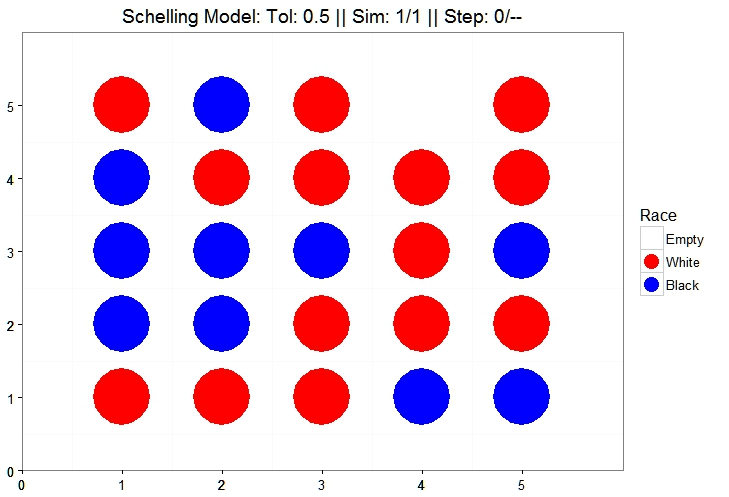
\includegraphics[scale=0.25]{figures/EX0.jpeg}
}
{%
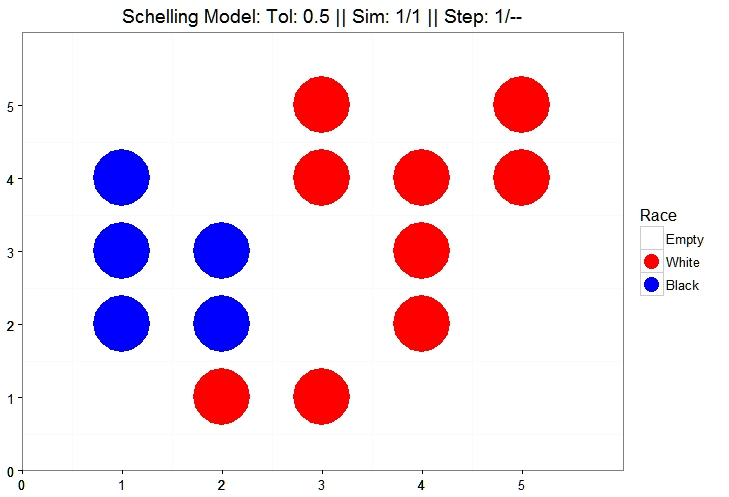
\includegraphics[scale=0.25]{figures/Ex1.jpeg}
}
{%
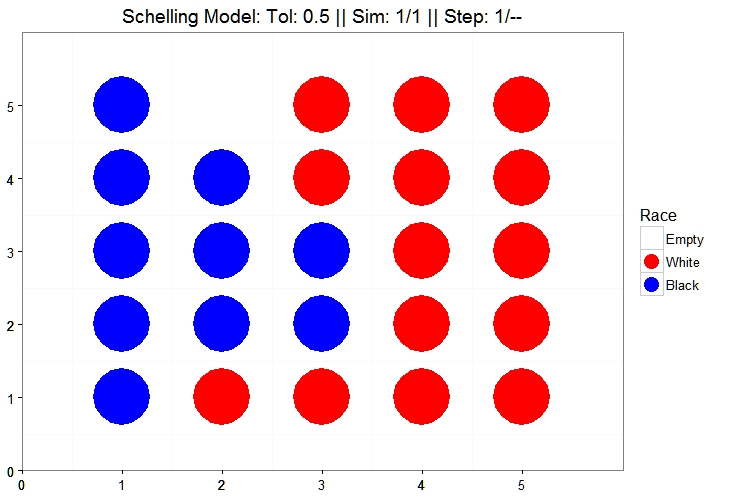
\includegraphics[scale=0.25]{figures/Ex2.jpeg}
}
\end{floatrow}
\caption[Example of Schelling Process]{Example of Schelling: $\tau = 50\%,\ M_{i=0} \rightarrow M_{i=2}$}
\end{figure}

The model in this paper adds a housing gradient as well as a wealth distribution to the original Schelling algorithm.

\section{Schelling with a Housing Market}

The housing market is a simple lottery. We take a housing price gradient as given from the data to rank the houses and rank the agents in order of wealth. The agents choose lexicographically with higher wealth agents choosing higher-priced houses. We look at the census tract data for median housing evaluation in Chicago for 2000 and 2010 to model the housing gradient. Spaces can also be empty, allowing the model to have neighborhoods that are more ``urban'' \textit{i.e.} have fewer empty dots, and to somewhat simulate urban decay. All this information is found in the 2000 and 2010 census tract data. Currently, the model does not attempt to simulate differing density levels. They may be done by using the continuous Schelling algorithm, however, this does slow the algorithm.

\begin{figure}[h!]
\centering
\begin{subfigure}{.45\textwidth}
  \centering
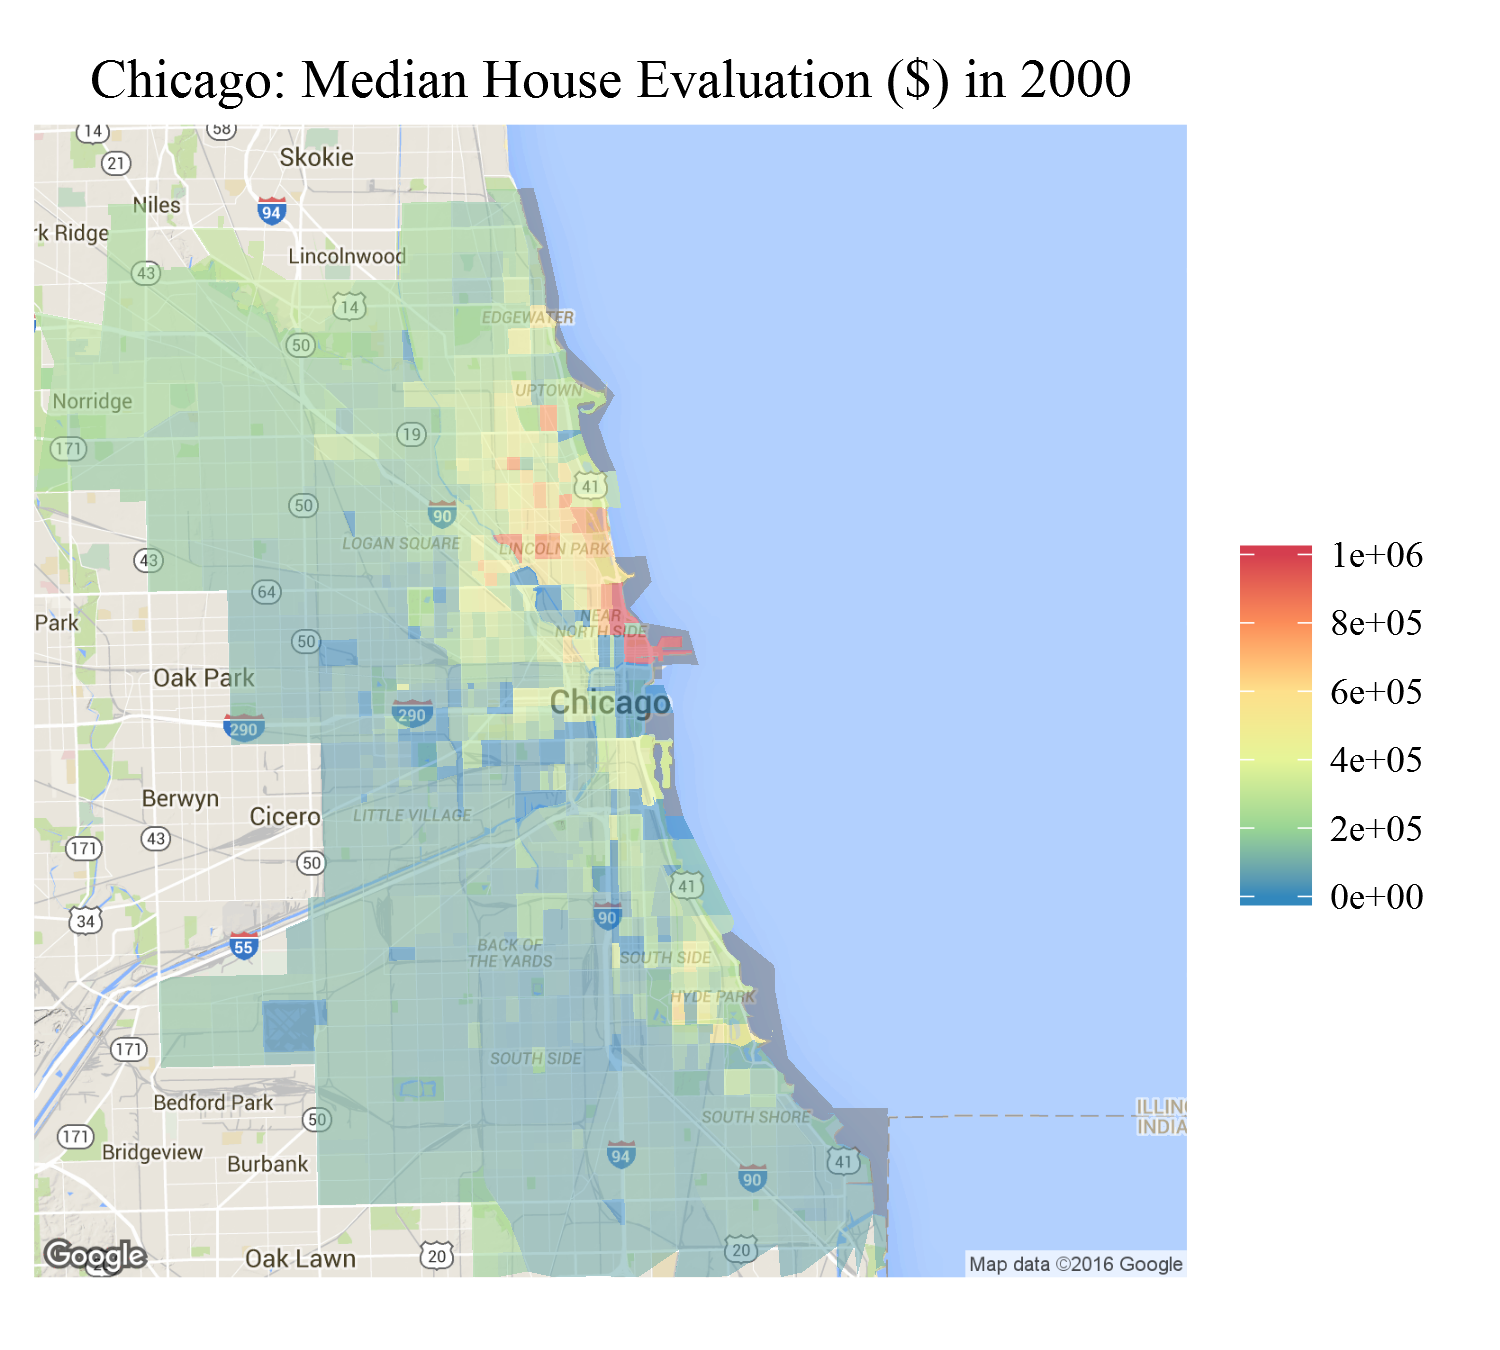
\includegraphics[scale=.15]{figures/c_2000.png}
\end{subfigure}%
\begin{subfigure}{.45\textwidth}
  \centering
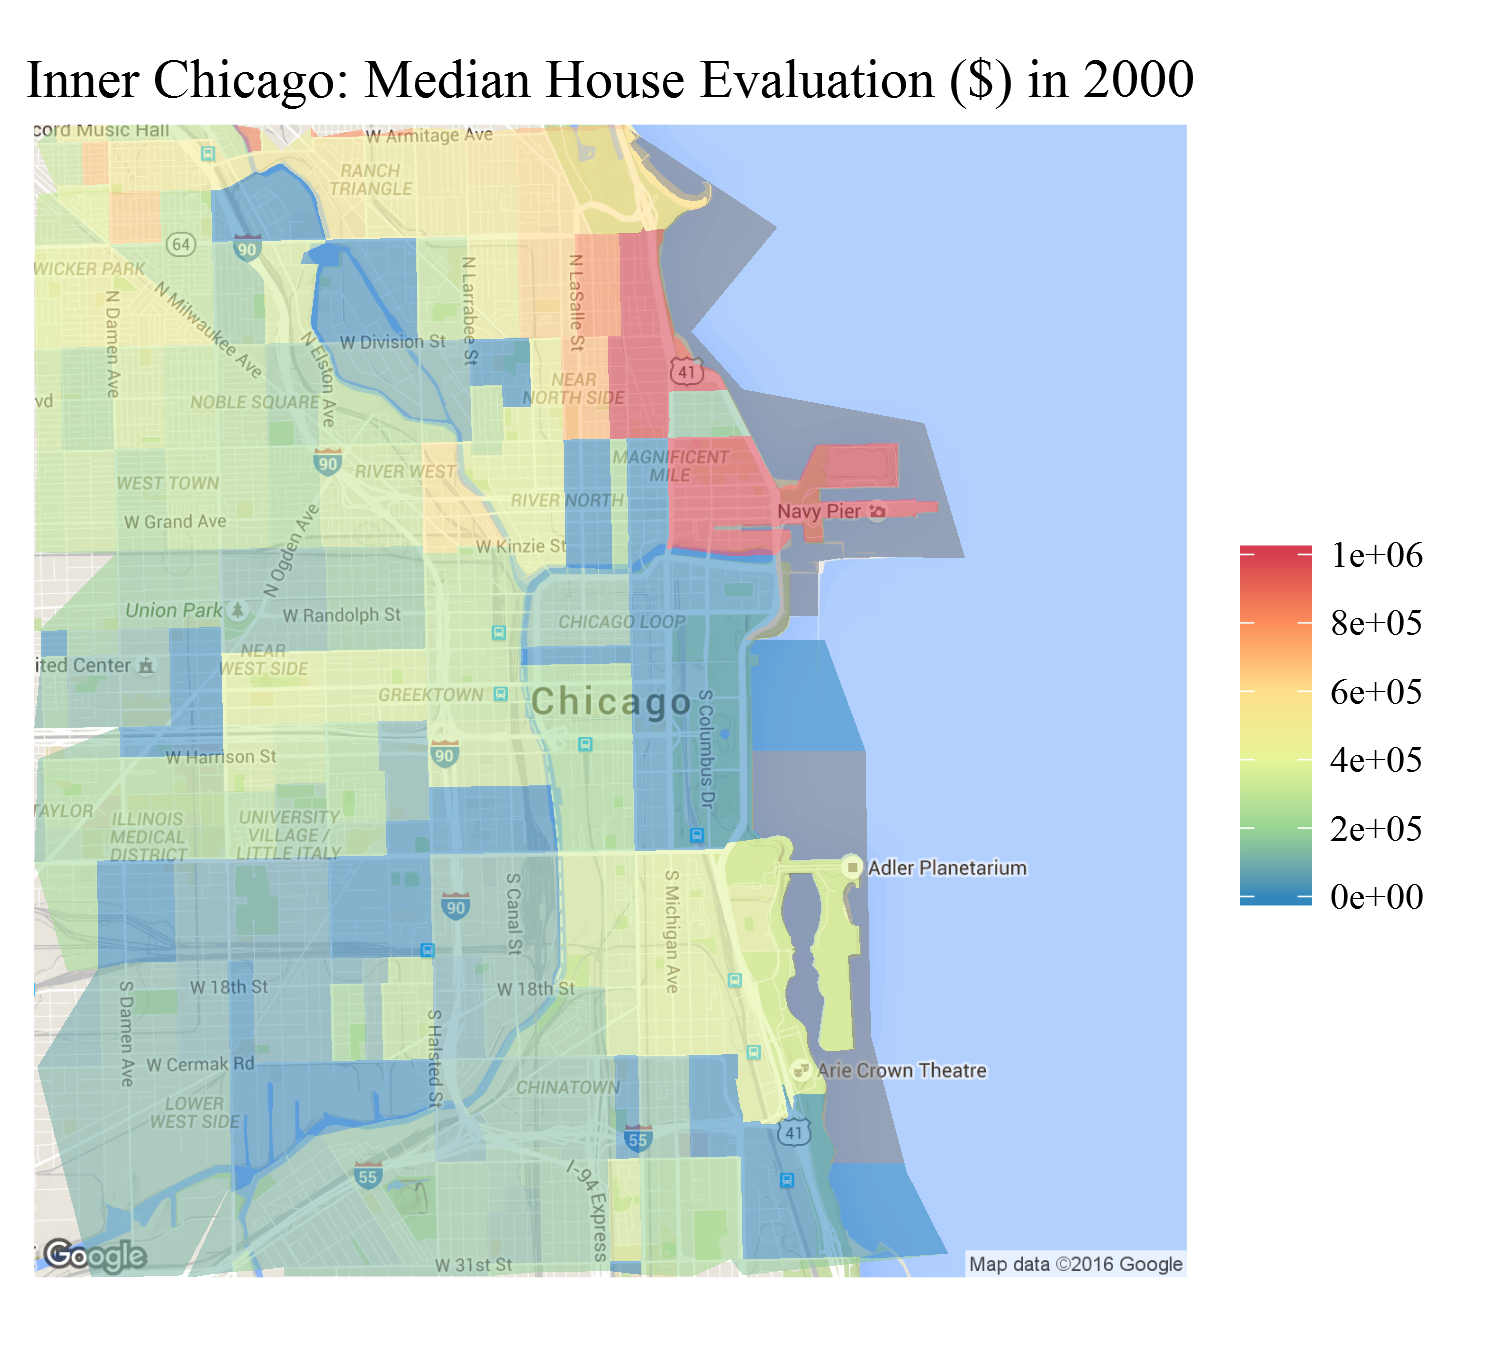
\includegraphics[scale=.15]{figures/c_2000_inner.png}
\end{subfigure}
\label{fig:chicago2000}
\begin{subfigure}{.45\textwidth}
  \centering
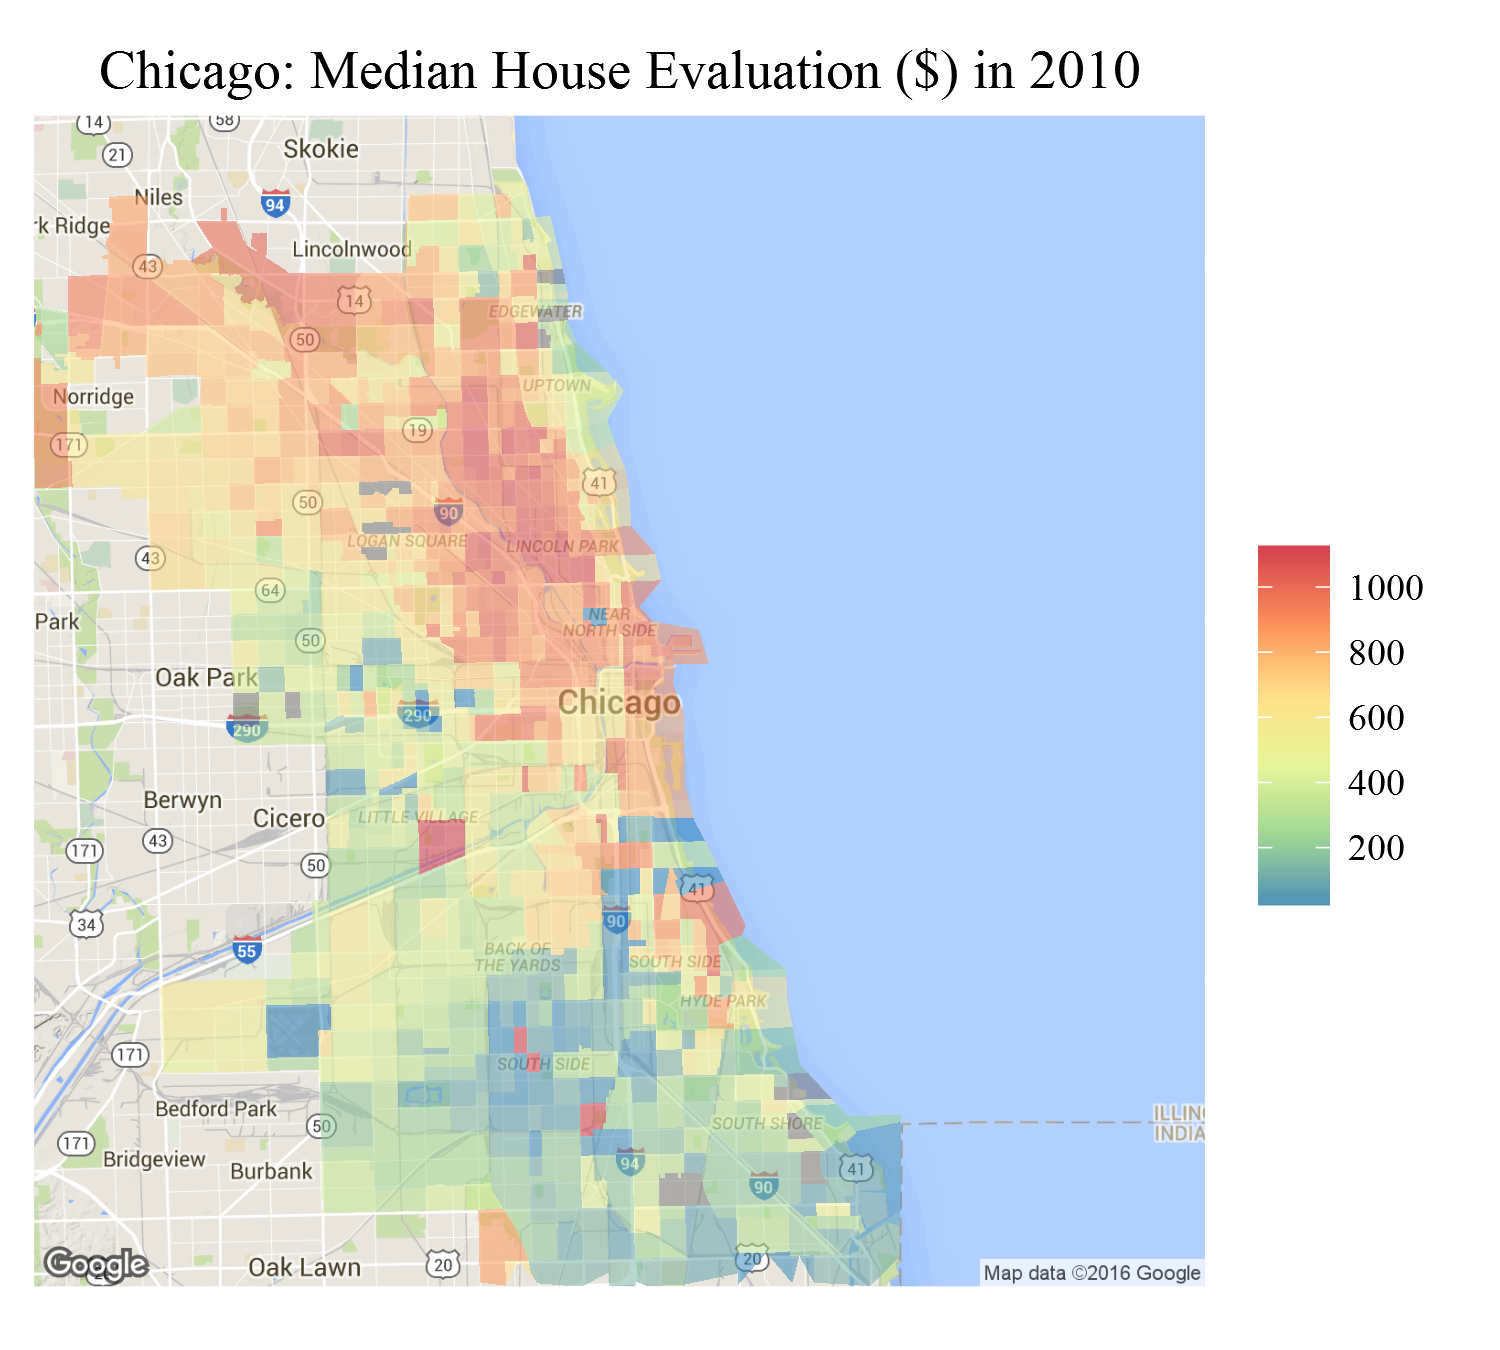
\includegraphics[scale=.15]{figures/c_2010.png}
\end{subfigure}%
\begin{subfigure}{.45\textwidth}
  \centering
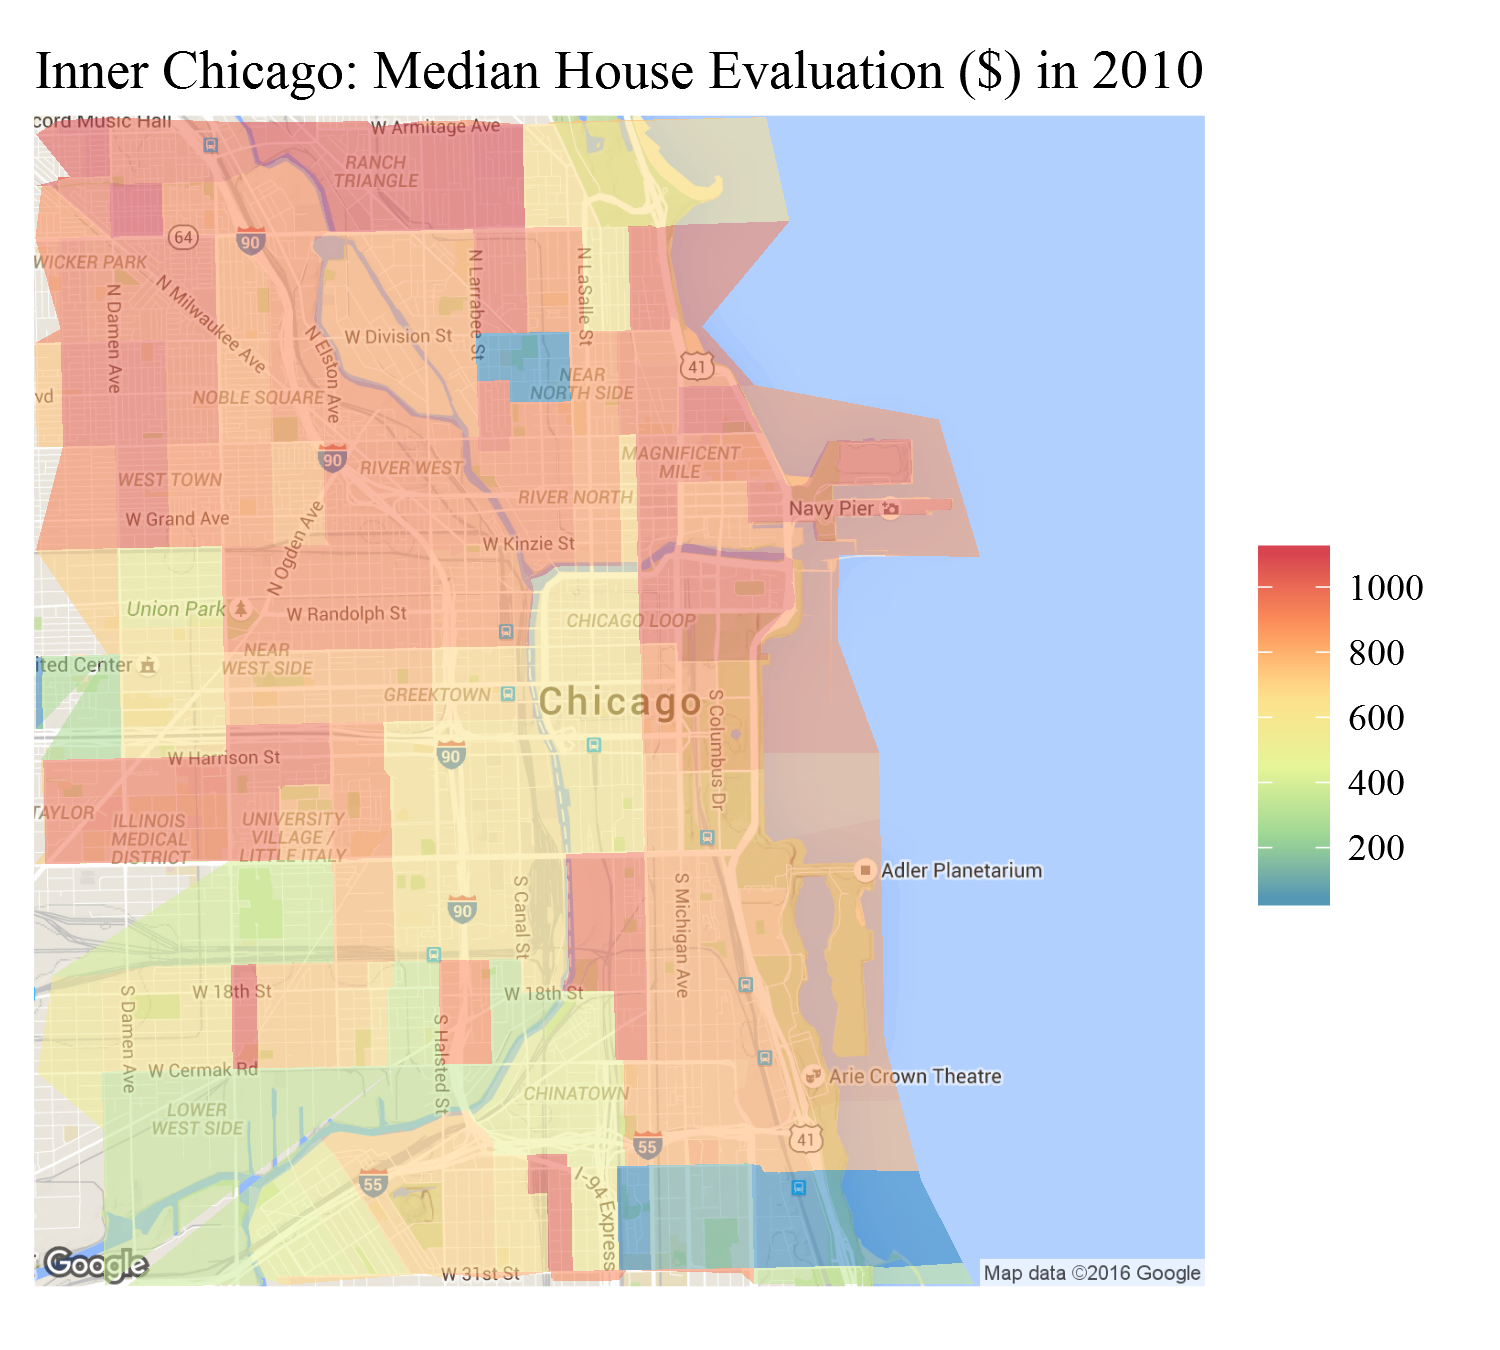
\includegraphics[scale=.15]{figures/c_2010_inner.png}
\end{subfigure}
\caption[Chicago Median Housing Evaluation, 2000-2010]{Chicago: Median Housing Evaluation (\$) in 2000 and 2010}
\label{fig:chicago2000}
\end{figure}

As one may note with Figure \ref{fig:chicago2000} below, the monocentric model of cities in urban economics roughly fits for Chicago \cite{brueckner87}. The center of the city is the most valued and house prices decay outward. However, within the city, there are several instances of high wealth next to low wealth. Urban Economists have a difficult time explaining why there is low wealth accumulation within the city center. Some researchers claim it is due to a combination of larger houses in the suburbs as well as access to better transportation \cite{glaeser08a}. The low wealth individual may only use public transportation while higher wealth individuals own their car(s). Both of these claims may be incorporated into the algorithm in future papers. This may be residual from the 1960s white flight where white people 'retreated' from the more mixed inner city neighborhoods to the mostly white suburbs. The algorithm developed in this paper may be used to analyze the transition, however, the algorithm is missing the structural racism that was present during this time period\cite{cutler97, cutler99}. Similarly, the algorithm is somewhat invariant to initial conditions\cite{zhang11}. It is not clear whether neighborhoods ought to be invariant or whether they are time dependent. Several authors have modeled the housing market with different lags and it is not clear how many lags a housing market may have\cite{glaeser07}. Other tipping algorithms have looked into studying this problem with mixed results\cite{card07}.

\begin{wrapfigure}{r}{.4\textwidth} %this figure will be at the right
    \centering
    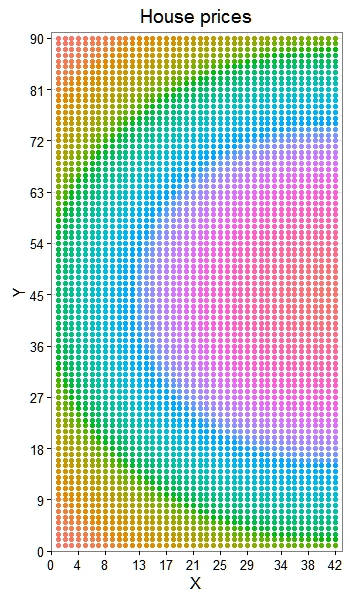
\includegraphics[scale=0.6]{figures/House_Price.jpeg}
    \caption[Simulated Housing Gradient Evaluation]{Simulated Housing Gradient Evaluation. More purple colors mean higher housing values. More red colors mean lower housing values. The decay in evaluation is defined by a euclidean distance}
\end{wrapfigure}


In 2010, the highest valued plot of land in Chicago moved northwest from the center. For now, we will assume that there is strict linear decay in the model for both 2000 and 2010. The housing gradient evaluation is simply a Euclidean distance from the center right of the plane. In future papers, one may need to construct a better fitting valuation gradient to better match the city being fitted. This paper does not analyze the robustness of precision of the price gradient. Similarly, upgrading the resolution using a Pointillist map may better capture the underlying distribution. This is especially true for cities which are currently gentrifying or have natural boundaries that create nonlinear (and/or even non-monotonic) price gradients. However, it is also worth noting that the housing market is only interested in ranking. Hence, changing the metric or the $2^{nd}$ derivative of price with respects to space should not change the ranking at all.

This paper modifies the algorithm to incorporate the housing market. Agents still only observe the race of other agents to determine whether they are satisfied. However, now \textit{unsatisfied} agents are sorted back lexicographically into the grid by their wealth. Specifically, agents are sorted by wealth and agents with higher wealth choose higher priced (or valued) houses. This process is described by Algorithm \ref{alg:extendschelling} below. This process allows for better clumping of wealthy agents. However, it allows for clumping of wealth agents in non-central locations. The complexity remains at $O(n^2)$ and there is not much change to the constant term in the complexity.

 \begin{algorithm}[htbp!]
  \caption{Extended Schelling Process}\label{alg:extendschelling}
  \begin{algorithmic}[1]
  	\Function{Extended Schelling}{$agents, grid, tolerance$}\Comment{Race and wealth define the agents.}
   		\Procedure{Satisfaction}{$agent_i, subgrid, tolerance$}\Comment{$subgrid$ is a Morse neighborhood of $agent_i$.}
        	\State Let $sat = \frac{\text{matching agents in $subgrid$ to $agent_i$}}{\text{size of subgrid}}$
       		\If {$tolerance < sat $}
       			\State return $TRUE$. \Comment{The agent is $satisfied$.}
                \Else \ return $FALSE$. \Comment{The agent is $unsatisfied$.}
    		\EndIf
        \EndProcedure
    	\While{for any $agent_i$, if Satisfaction is FALSE}
        	\State Remove all $unsatisfied$ agents from grid.
            \State Rank all $unsatisfied$ agents by wealth.
            \State Rank all grid spots by the housing price index.
            \State Place all $unsatisfied$ agents in order of wealth to the most valuable real estate on grid.
        \EndWhile{}
  	\EndFunction{}
  \end{algorithmic}
  \end{algorithm}
  \begin{figure}[h!]
\caption{Algorithm of Extended Schelling Process}
\end{figure}

\begin{figure}[h!]
\centering
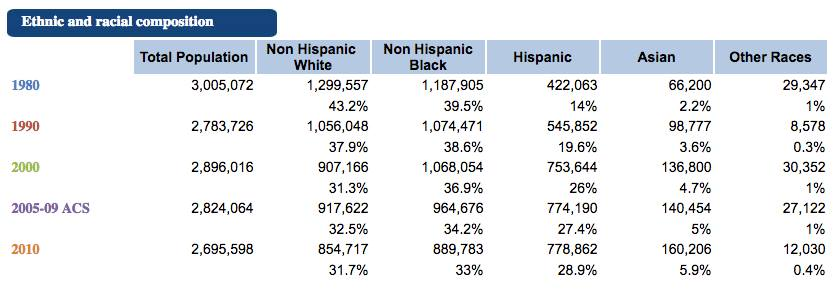
\includegraphics[scale=0.5]{figures/chart4.png}
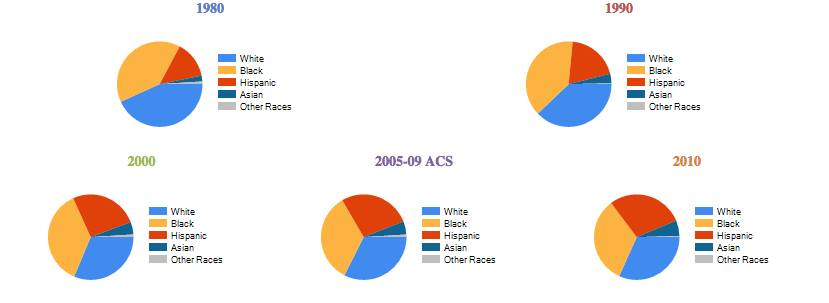
\includegraphics[scale=0.4]{figures/chart3.png}
\caption[Demographics of Chicago]{Demographics of Chicago (Source: US2010)\cite{brown10}}
\label{tab:chicago2}
\end{figure}


The extended Schelling algorithm, by virtue of incorporating both race and wealth, requires a distribution of race and wealth within the population. In fact, the extended algorithm allows for some nuance in the distribution, including individual wealth distribution by race. This allows the extended Schelling algorithm to incorporate the significant wealth differences between races. Figure \ref{tab:chicago2} shows the racial makeup of Chicago in 2000 and 2010. Table \ref{tab:chicago} shows the adjusted racial and wealth make up of Chicago in 2000 and 2010 for the simulation. Races with less than 10\% of the population were dropped as Schelling has difficulty modeling with such low numbers. The wealth distribution represents the fraction of individuals with wealth in the categories described by $w(x)$ in Equation \ref{eq:w}. Note that incomes generally moved up. These incomes, however, are not adjusted for inflation. Census tracts only provide ranges of income, so there is no way to correct for inflation because there is not enough resolution to correctly adjust the category of the edge cases. However, noting that all races saw about 5\% of the population move from income 1 to income 2, it is likely that inflation accounts for much of this change. This effect is different for Whites than for nonwhites, however. Nonwhites saw about 5\% of individuals move from income 2 to income 3, but Whites saw nearly 15\% make that jump.

\begin{table}[h!]
\centering
\caption{Demographics of Chicago}
\label{tab:chicago}
\scalebox{1}{
\begin{tabular}{lllll}
\hline
\multicolumn{5}{l}{Demographics of Chicago Used in Simulations}                                                        \\ \hline \hline
\multicolumn{1}{l|}{Year}     & \multicolumn{2}{l|}{2000}                       & \multicolumn{2}{l}{2010}   \\ \hline
\multicolumn{1}{l|}{Race}     & Population Ratio & \multicolumn{1}{l|}{Wealth Distribution}  & Population Ratio & Wealth Distribution  \\
\multicolumn{1}{l|}{White}    & 60\%           & \multicolumn{1}{l|}{30\%|50\%|20\%} & 56\%            & 25\%|41\%|34\%  \\
\multicolumn{1}{l|}{Black}    & 26\%           & \multicolumn{1}{l|}{53\%|40\%|07\%} & 27\%            & 49\%|40\%|11\%  \\
\multicolumn{1}{l|}{Hispanic} & 14\%           & \multicolumn{1}{l|}{43\%|50\%|07\%} & 17\%            & 37\%|51\%|12\%  \\ \hline \hline
\end{tabular}
}
\end{table}

Other than the significant increase in White wealth, the demographics of Chicago show mostly stable trends from 2000 to 2010. There is a 5\% upwards income drift and a slight decrease in the white population as a share. Asians and other small mass races are excluded from this analysis; the population ratio is the ratio of Chicago's White, Black, and Hispanic population, not the share of its total population. By simulating Chicago with the 2000 and 2010 demographics, one can see whether similar tolerance levels reproduce Chicago's actual segregation statistics on average. If the tolerance level $\tau$ decreases, then this simulation would be evidence of Chicago becoming more racially tolerant. 

